\documentclass[12pt, oneside]{article}

\usepackage[letterpaper, scale=0.8, centering]{geometry}
\usepackage{fancyhdr}
\setlength{\parindent}{0em}
\setlength{\parskip}{1em}

\pagestyle{fancy}
\fancyhf{}
\renewcommand{\headrulewidth}{0pt}
\rfoot{{\footnotesize Copyright Mia Minnes, 2025, Version \today~(\thepage)}}

\usepackage{titlesec}

\author{CSE105W25}

\newcommand{\instructions}{{\bf For all HW assignments:} Weekly homework 
may be done individually or in groups of up to 3 students. 
You may switch HW partners for different HW assignments. 
Please ensure your name(s) and PID(s) are clearly visible on the first page of your homework submission 
and then upload the PDF to Gradescope. If working in a group, submit only one submission per group: 
one partner uploads the submission through their Gradescope account and then adds the other group member(s) 
to the Gradescope submission by selecting their name(s) in the ``Add Group Members" dialog box. 
You will need to re-add your group member(s) every time you resubmit a new version of your assignment.
 Each homework question will be graded either for correctness (including clear and precise explanations and 
 justifications of all answers) or fair effort completeness. 
 On the ``graded for correctness"
 questions, you may only collaborate with CSE 105 students in your group; if your
 group has questions about a problem, you may ask in drop-in help hours or post a private
post (visible only to the Instructors) on Piazza. On the "graded for completeness" questions, you 
may collaborate with all other CSE 105 students this quarter, and you may make public posts about these questions 
on Piazza.

All submitted homework for this class must be typed. 
You can use a word processing editor if you like (Microsoft Word, Open Office, Notepad, Vim, Google Docs, etc.) 
but you might find it useful to take this opportunity to learn LaTeX. 
LaTeX is a markup language used widely in computer science and mathematics. 
The homework assignments are typed using LaTeX and you can use the source files 
as templates for typesetting your solutions.
To generate state diagrams of machines, you can (1) use the LaTex tikzpicture
environment (see templates in the class notes), or (2) use the software tools Flap.js or
JFLAP described in the class syllabus (and include a screenshot in your PDF), or (3) you can carefully
and clearly hand-draw
the diagram and take a picture and include it in your PDF.
We recommend that you
submit early drafts to Gradescope so that in case of any technical difficulties, at least some of your
work is present. You may update your submission as many times as you'd like up to the deadline.


{\bf Integrity reminders}
\begin{itemize}
\item Problems should be solved together, not divided up between the partners. The homework is
designed to give you practice with the main concepts and techniques of the course, 
while getting to know and learn from your classmates.
\item On the "graded for correctness"
questions, you may only collaborate with CSE 105 students in your group.
You may ask questions about the homework in office hours (of the instructor, TAs, and/or tutors) and 
on Piazza (as private notes viewable only to the Instructors).  
You \emph{cannot} use any online resources about the course content other than the class material 
from this quarter -- this is primarily to ensure that we all use consistent notation and
definitions (aligned with the textbook) and also to protect the learning experience you will have when
the `aha' moments of solving the problem authentically happen.
\item Do not share written solutions or partial solutions for homework with 
other students in the class who are not in your group. Doing so would dilute their learning 
experience and detract from their success in the class.
\end{itemize}

}

\newcommand{\gradeCorrect}{({\it Graded for correctness}) }
\newcommand{\gradeCorrectFirst}{\gradeCorrect\footnote{This means your solution 
will be evaluated not only on the correctness of your answers, but on your ability
to present your ideas clearly and logically. You should explain how you 
arrived at your conclusions, using
mathematically sound reasoning. Whether you use formal proof techniques or 
write a more informal argument
for why something is true, your answers should always be well-supported. 
Your goal should be to convince the
reader that your results and methods are sound.} }
\newcommand{\gradeComplete}{({\it Graded for completeness}) }
\newcommand{\gradeCompleteFirst}{\gradeComplete\footnote{This means you will 
get full credit so long as your submission demonstrates honest effort to 
answer the question. You will not be penalized for incorrect answers. 
To demonstrate your honest effort in answering the question, we 
expect you to include your attempt to answer *each* part of the question. 
If you get stuck with your attempt, you can still demonstrate 
your effort by explaining where you got stuck and what 
you did to try to get unstuck.} }

\usepackage{tikz}
\usetikzlibrary{automata,positioning,arrows}

\usepackage{amssymb,amsmath,pifont,amsfonts,comment,enumerate,enumitem}
\usepackage{currfile,xstring,hyperref,tabularx,graphicx,wasysym}
\usepackage[labelformat=empty]{caption}
\usepackage{xcolor}
\usepackage{multicol,multirow,array,listings,tabularx,lastpage,textcomp,booktabs}

\lstnewenvironment{algorithm}[1][] {   
    \lstset{ mathescape=true,
        frame=tB,
        numbers=left, 
        numberstyle=\tiny,
        basicstyle=\rmfamily\scriptsize, 
        keywordstyle=\color{black}\bfseries,
        keywords={,procedure, div, for, to, input, output, return, datatype, function, in, if, else, foreach, while, begin, end, }
        numbers=left,
        xleftmargin=.04\textwidth,
        #1
    }
}
{}

\newcommand\abs[1]{\lvert~#1~\rvert}
\newcommand{\st}{\mid}

\newcommand{\cmark}{\ding{51}}
\newcommand{\xmark}{\ding{55}}
 
\newcommand{\SUBSTRING}{\textsc{Substring}}
\newcommand{\REP}{\textsc{Rep}}
\newcommand{\blank}{\scalebox{1.5}{\textvisiblespace}}
 
\title{HW2CSE105W25: Homework assignment 2}
\date{Due: January 30th at 5pm, via Gradescope}


\begin{document}
\maketitle
\thispagestyle{fancy}

{\bf In this assignment,}

You will practice designing multiple representations of regular languages and working with 
general constructions of automata to demonstrate the richness of the class of regular languages.


{\bf Resources}: To review the topics 
for this assignment, see the class material from Week 2 and Week 3.
We will post frequently asked questions and our answers to them in a 
pinned Piazza post. 

{\bf Reading and extra practice problems}:  
Sipser Section 1.1, 1.2, 1.3. 
Chapter 1 exercises 1.4, 1.5, 1.6, 1.7, 1.8, 1.9, 1.10, 1.11, 1.12, 1.13, 1.14, 1.15, 
1.16, 1.17, 1.18, 1.19, 1.20, 1.21, 1.22, 1.23. Chapter 1 problem 1.31, 
1.36, 1.37.

\instructions

You will submit this assignment via Gradescope
(\href{https://www.gradescope.com}{https://www.gradescope.com}) 
in the assignment called ``hw2CSE105W25''.

{\bf Assigned questions}
\begin{enumerate}[wide, labelwidth=!, labelindent=0pt]
\item\textbf{Finite automata} (10 points):
Consider the finite automaton $M = (Q, \Sigma, \delta, q_0, F)$ whose state diagram is depicted below
\begin{center}
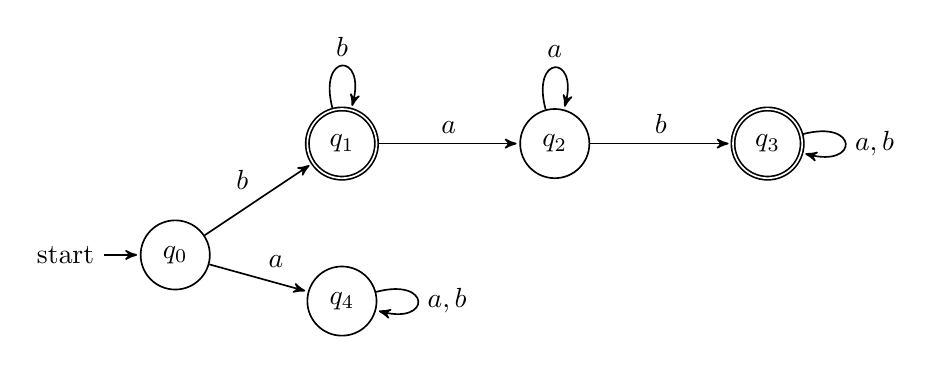
\begin{tikzpicture}[->,>=stealth',shorten >=1pt, auto, node distance=2cm, semithick]
\tikzstyle{every state}=[text=black, fill=none]

\node[initial,state] (q0)          {$q_0$};
\node[state,accepting]         (q1) [above right of=q0, xshift=20pt] {$q_1$};
\node[state]         (q2) [right of=q1, xshift=20pt] {$q_2$};
\node[state,accepting]         (q3) [right of=q2, xshift=20pt] {$q_3$};
\node[state] (q4) [below of=q1] {$q_4$};

\path (q0) edge  [bend left=0] node {$b$} (q1)
        edge [bend left=0] node{$a$} (q4)
    (q1) edge [loop above] node {$b$} (q1)
        edge [bend left=0] node {$a$} (q2)
    (q2) edge [bend left=0] node {$b$} (q3)
        edge [loop above] node {$a$} (q2)
    (q3) edge [loop right] node {$a,b$} (q3)
    (q4) edge [loop right] node{$a,b$} (q4)
;
\end{tikzpicture}
\end{center}
    \begin{enumerate}
    \item\gradeCompleteFirst Write the formal definition of this automaton. In other words, give the five defining paramaters $Q$, $\Sigma$, $\delta$, $q_0$, $F$ so that they are consistent with the state diagram of $M$.

    \item\gradeCorrectFirst Give a regular expression $R$ so that $L(R) = L(M)$. In other words, we want a regular expression that describes the language 
    recognized by this finite automaton. Justify your answer by referring to the 
    definition of the semantics of regular expressions and computations of finite automata. 
    Include an explanation for why each string in $L(R)$ is accepted by the finite automaton {\it and}
    for why each string not in $L(R)$ is rejected by the finite automaton.

    {\it Ungraded bonus: can you find more than one such regular expression?}

    \item\gradeComplete Keeping the same set of states $Q$, 
    input alphabet $\Sigma$, 
    same start state $q_0$, and same transition 
    function $\delta$, choose a new set of accepting states $F_{new1}$ so that the new 
    finite automaton $M_1 = (Q, \Sigma, \delta, q_0, F_{new1})$ that results 
    recognizes a {\bf proper superset} of $L(M)$, or explain 
    why there is no such example. 
    A complete solution will include either (1) a precise and
    clear description of your choice of $F_{new1}$
    {\it and} a precise and clear explanation of why every string that is accepted by 
    $M$ is also accepted by $M_1$ {\it and} an example of a string that is accepted by $M_1$ and is rejected by $M$; or (2) a sufficiently general and correct argument
    why there is no such example, referring back to the relevant definitions.


    \item\gradeCorrect Keeping the same set of states $Q$, 
    input alphabet $\Sigma$, 
    same start state $q_0$, and same transition 
    function $\delta$, choose a new set of accepting states $F_{new2}$ so that the new 
    finite automaton $M_2 = (Q, \Sigma, \delta, q_0, F_{new2})$ that results 
    recognizes a {\bf nonempty proper subset} of $L(M)$, or explain 
    why there is no such example. 
    A complete solution will include either (1) a precise and
    clear description of your choice of $F_{new2}$
    {\it and} an example string accepted by $M_2$ {\it and} a precise and clear explanation of why every string that is accepted by 
    $M_2$ is also accepted by $M$ {\it and} an example of a string that is accepted by $M$ and is rejected by $M_2$; or (2) a sufficiently general and correct argument
    why there is no such example, referring back to the relevant definitions.

    \end{enumerate}

\item \textbf{Automata design} (12 points):
As background to this question, recall that integers can be represented using base $b$ expansions, for 
any convenient choice of base $b$. The precise definition is:
for $b$ an integer greater than $1$ and $n$ a positive integer, 
the {\bf base $b$ expansion of $n$}  is defined to be
\[
(a_{k-1} \cdots a_1 a_0)_b
\]
where $k$ is a positive integer, $a_0, a_1, \ldots, a_{k-1}$ 
are nonnegative integers less than $b$, $a_{k-1} \neq  0$, and
\[
n =  \sum_{i=0}^{k-1} a_{i} b^{i}
\]

Notice: {\it The base $b$ expansion of a positive integer $n$ is a string over the alphabet 
$\{x \in \mathbb{Z} \st 0 \leq x < b\}$
whose leftmost character is nonzero.}

An important property of base $b$ expansions of integers is that, for each integer $b$ greater than $1$,
each positive integer $n = (a_{k-1} \cdots a_1 a_0)_b$, and each nonnegative integer $a$ less than $b$, 
\[
    bn + a = (a_{k-1} \cdots a_1 a_0a)_b
\]
In other words, shifting the base $b$ expansion to the left results in multiplying the integer value by the base.
In this question we'll explore building deterministic finite automata that recognize 
languages that correspond to useful sets of integers.

    \begin{enumerate}
    \item\gradeComplete Design a DFA that recognizes the set of binary (base $2$) expansions of 
    positive integers that are powers of $2$. A complete solution will include the state diagram of your DFA and 
    a brief justification 
    of your construction by explaining the role each state plays in the machine, as well as a brief 
    justification about how the strings accepted and rejected by the machine connect to the specified language.

    {\it Hints}: (1) A power of $2$ is an integer $x$ that can be written as $2^y$ for some nonnegative integer $y$, 
    (2) the DFA should accept the strings $100$, $10$ and $100000$ and should reject the 
    strings $010$, $1101$, and $\varepsilon$ (can you see why?).

    \item\gradeCorrect Design a DFA that recognizes the set of 
    binary (base $2$) expansions of positive integers that are less than $10$. Your DFA must use {\bf fewer than ten states}. 
    A complete solution will include the state diagram of your DFA and 
    a brief justification 
    of your construction by explaining the role each state plays in the machine, as well as a brief 
    justification about how the strings accepted and rejected by the machine connect to the specified language.

    \item \gradeComplete Find a positive integer $B$ greater than $1$ so that 
    there is a DFA that recognizes the set of 
    base $B$ expansions of positive integers that are less than $10$ and it 
    uses as few states as possible. A complete solution will include the state 
    diagram of your DFA and 
    a brief justification of your choice of base.
        

    {\it Hint: sometimes rewriting the defining membership condition for a set in different ways helps us find alternate representations of that set.}
    \end{enumerate}


\item \textbf{Nondeterminism} (15 points): For this question, the alphabet is $\{a,b,c\}$.
\begin{enumerate}
\item\gradeComplete Design a NFA that recognizes the language
    \[ 
    L_1 = \{w \in \{a,b,c\}^* \mid w \text{ starts with $a$ {\bf and} ends with $a$}\}
    \]

    A complete solution will include the state diagram of your NFA and 
    a brief justification 
    of your construction that explains the role each state plays in the machine, as well as a brief 
    justification about how the strings accepted and rejected by the machine connect to the specified language.

\item\gradeCorrect Design a NFA that recognizes the language 
    \[ 
    L_2 = \{w \in \{a,b,c\}^* \mid w \text{ has no consecutive repeated characters}\}
    \]
    For example, the empty string, $a$, $bac$, and $abca$ are each elements of this language but $aa$ and $abb$ and $abbc$ are not elements of this language.

    A complete solution will include the state diagram of your NFA and 
    a brief justification 
    of your construction that explains the role each state plays in the machine, as well as a brief 
    justification about how the strings accepted and rejected by the machine connect to the specified language.

\item\gradeComplete Consider the language
\begin{align*}
L_1 \cup L_2 = \{w \in \{a,b,c\}^* \mid w &\text{ starts with $a$ and ends with $a$} \\
&\text{{\bf or} has no consecutive repeated characters}\}
\end{align*}
Give at least two representations of this language among the following: 
\begin{itemize}
\item A regular expression that describes $L_1 \cup L_2$
\item A DFA that recognizes $L_1 \cup L_2$
\item A NFA that recognizes $L_1 \cup L_2$
\end{itemize}

You can design your automata directly or use the constructions from class and chapter 1 in the book to build these automata from automata for the simpler languages.
    
A complete solution will include at least two of the representations
as well as  a brief justification of each construction.


\item\gradeComplete Consider the language
    \begin{align*}
    L_1 \cap L_2 = \{w \in \{a,b,c\}^* \mid w &\text{ starts with $a$ and ends with $a$} \\
    &\text{{\bf and} has no consecutive repeated characters}\}
    \end{align*}
    Give at least two representations of this language among the following: 
    \begin{itemize}
    \item A regular expression that describes $L_1 \cap L_2$
    \item A DFA that recognizes $L_1 \cap L_2$
    \item A NFA that recognizes $L_1 \cap L_2$
    \end{itemize}
    You can design your automata directly or use the constructions from class and chapter 1 in the book to build these automata from automata for the simpler languages.
    
A complete solution will include at least two of the representations
as well as  a brief justification of each construction.

\end{enumerate}

\item\textbf{General constructions} (13 points):
In this question, you'll practice working with formal general constructions
for automata and translating between state diagrams and formal definitions.


Recall the definitions of operations we've talked about that produce
new languages from old: for each language $L$ over an alphabet $\Sigma$, 
we have the 
associated sets of strings (also over $\Sigma$)
\[
    L^* = \{ w_1 \cdots w_k \mid k \geq 0 \textrm{ and each } w_i \in L\}
\]
and
\[
    SUBSTRING(L) = \{ w \in \Sigma^* ~|~ \text{there exist } x,y \in \Sigma^* \text{ such that } xwy \in L\}
\]
and 
\[
    EXTEND(L) = \{ w \in \Sigma^* ~|~ w = uv \text{ for some strings } u \in L \text{ and } v \in \Sigma^* \}
\]
Also, recall the set operations union and intersection: for any sets $X$ and $Y$
\[
X \cup Y = \{ w \mid w \in X \text{ or } w \in Y \}
\]
\[
X \cap Y = \{ w \mid w \in X \text{ and } w \in Y \}
\]


Let $M_1 = (Q_1, \Sigma, \delta_1, q_1, F_1)$ and 
$M_2 = (Q_2, \Sigma, \delta_2, q_2, F_2)$ be DFA.

For simplicity, assume that $Q_1 \cap Q_2 = \emptyset$ and that 
$q_0 \notin Q_1 \cup Q_2$.

Consider the following definitions of new automata parameterized by 
these DFA:
\begin{itemize}
\item The NFA $N_\alpha = ( Q_1 \cup Q_2 \cup \{q_0\}, \Sigma, \delta_\alpha, q_0, F_1 \cup F_2)$ with the transition function given by 
\[
\delta_\alpha ( ~(q,x)~) = \begin{cases}
\{q_1, q_2\} &\text{if $q = q_0$, $x = \varepsilon$} \\
\emptyset &\text{if $q=q_0$, $x\in \Sigma$}\\
\{\delta_{1}(~(q,x)~)\} &\text{if $q\in Q_1$, $x\in \Sigma$}\\
\{\delta_{2}(~(q,x)~)\} &\text{if $q\in Q_2$, $x\in \Sigma$}\\
\emptyset &\text{if $q \in Q_1 \cup Q_2$, $x = \varepsilon$} \\
\end{cases}
\]
\item The NFA $N_\beta = ( Q_1 \times Q_2, \Sigma, \delta_\beta, (q_1,q_2), F_1 \times F_2)$  with the transition function given by 
\[
\delta(~(~(r,s)~, x~)~) = \{ (~\delta_{1}(~(r,x)~), \delta_{2}( ~(s,x)~)~)\}
\]
 and 
\[
\delta(~(~(r,s)~, \varepsilon~)~) = \emptyset
\]
for $r \in Q_1, s \in Q_2, x \in \Sigma$.
\item The NFA $N_{\gamma}=(Q_1\cup\{q_{0}\},\Sigma,\delta_{\gamma},q_{0},\{q \in Q_1 \mid \exists w \in \Sigma^* (\delta_1^* ((q,w)) \in F_1)\})$, and
        \[
            \delta_{\gamma} ((q,a)) = \begin{cases}
                \{\delta_1((q,a))\} &\text{if $q \in Q_1$, $a \in \Sigma$} \\
                \{q' \in Q_1 \mid \exists w \in \Sigma^* (\delta_1^*((q_1,w)) = q') \}&\text{if $q =q_{0}$, $a = \varepsilon$}\\
                \emptyset &\text{if $q = q_{0}$, $a \in \Sigma$} \\
                \emptyset &\text{if $q \in Q_1$, $a = \varepsilon$}
            \end{cases}
        \]

{\it Hint: the notation $\delta_1^*$ refers to the iterated transition function.}
\end{itemize}



\begin{enumerate}
\item\gradeCorrect 
Illustrate the construction of $N_{\alpha}$ by defining a specific pair 
of example DFAs $M_1$ and $M_2$ and applying the 
construction above to create the new NFA $N_\alpha$. Your example DFA should
\begin{itemize}
    \item Have the same input alphabet as each other, 
    \item Each have exactly three states (all reachable from the respective start state),
    \item Accept at least one string and reject at least one string, 
    \item Recognize different languages from one another, and
    \item Not have any states labelled $q_0$, and 
    \item Not share any state labels.
\end{itemize}
Apply the construction above to create the new NFA. A complete submission 
will include the state diagrams of your example DFA $M_1$ and $M_2$ and the state diagram of the NFA $N_\alpha$ resulting 
from this construction and a precise and clear description of $L(M_1)$ and $L(M_2)$ and $L(N_{\alpha})$, justified
by explaining the role each state plays in the machine, as well as a brief 
justification about how the strings accepted and rejected by the machine connect to the language.

\item\gradeCorrect 
Illustrate the construction of $N_{\beta}$ by defining a specific pair 
of example DFAs $M_1$ and $M_2$ and applying the 
construction above to create the new NFA $N_\beta$. Your example DFA should
\begin{itemize}
    \item Have the same input alphabet as each other, 
    \item Each have exactly two states (all reachable from the respective start state),
    \item Accept at least one string and reject at least one string, 
    \item Recognize different languages from one another, and
    \item Not have any states labelled $q_0$, and 
    \item Not share any state labels.
\end{itemize}
Apply the construction above to create the new NFA. A complete submission 
will include the state diagrams of your example DFA $M_1$ and $M_2$ and the state diagram of the NFA $N_\beta$ resulting 
from this construction and a precise and clear description of $L(M_1)$ and $L(M_2)$ and $L(N_{\beta})$, justified
by explaining the role each state plays in the machine, as well as a brief 
justification about how the strings accepted and rejected by the machine connect to the language.


\item\gradeCorrect 
Illustrate the construction of $N_{\gamma}$ by defining a specific
example DFA $M_1$  and applying the 
construction above to create the new NFA $N_\gamma$. Your example DFA should
\begin{itemize}
    \item Have exactly four states (all reachable from the respective start state),
    \item Accept at least one string and reject at least one string, 
    \item Not have any states labelled $q_0$.
\end{itemize}
Apply the construction above to create the new NFA. A complete submission 
will include the state diagram of your example DFA $M_1$ and the state diagram of the NFA $N_\gamma$ resulting 
from this construction and a precise and clear description of $L(M_1)$ and $L(N_{\gamma})$, justified
by explaining the role each state plays in the machine, as well as a brief 
justification about how the strings accepted and rejected by the machine connect to the language.

\item \gradeComplete If possible, associate each construction above with one of the operations whose definitions we recalled at the start of the question.  For example, is it the case that (for all choices of DFA $M_1$ and $M_2$) $L(N_\alpha) = L(M_1) \cup L(M_2)$? or $L(N_\alpha) = L(M_1) \cap L(M_2)$? etc.

A complete solution will consider each of the constructions $N_\alpha, N_\beta, N_\gamma$ in turn, and for each, either name the operation that's associated with the construction (and explain why) or explain why none of the operations mentioned is associated with the construction.
\end{enumerate}

\end{enumerate}
\end{document}